\section{Procedimento \& Analisi Dati}

Nell'ottica geometrica si usano le leggi del costruttore di lenti e dei punti coniugati.
Tali leggi si basano sulle ipotesi di raggi parassiali e lenti sottili, che dobbiamo quindi supporre verificate
nel nostro apparato sperimentale. Una parte dell'esperienza, quella relativa alle due tipologie di aberrazione, è dedicata alla misura dei limiti di tali approssimazioni.

\begin{figure}[b!]
	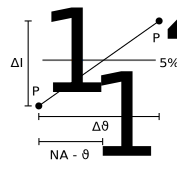
\includegraphics[width=16cm]{drawing.pdf}
    \caption{Schema dell'apparato sperimentale usato per la misura del fuoco della lente convergente.}
    \label{fig:conv}
\end{figure}

\subsection{Fuoco della lente convergente}

Per non appesantire la lettura, nel seguito indicheremo con queste lettere le seguenti quantità (si veda la Figura \ref{fig:conv}):

\begin{equation*}
	p \,=\, \text{distanza tra il centro della lente e la posizione dell'oggetto}
\end{equation*}
\begin{equation*}
	q \,=\, \text{distanza tra il centro della lente e la posizione dell'immagine}
\end{equation*}
\begin{equation*}
	f \,=\, \text{fuoco della lente analizzata}
\end{equation*}
\begin{equation*}
	h \ped{imm} \,=\, \text{altezza dell'immagine sullo schermo}
\end{equation*}
%\begin{equation}
%	\text{Legge dei punti coniugati:} \qquad \frac{1}{f} \,=\, \frac{1}{p} + \frac{1}{q}
%	\label{eq:coniugati}
%\end{equation}
%\begin{equation}
%	\text{Legge del costruttore di lenti:} \qquad \frac{1}{f} \,=\, (n-1)\left(\frac{1}{R\ped{1}}-\frac{1}{R\ped{2}}\right)
%	\label{eq:costruttore}
%\end{equation}


Come primo obiettivo ci siamo posti di calcolare il fuoco e l'ingrandimento della lente convergente per diversi valori di $p$ e $q$. Abbiamo quindi misurato dodici valori di $q$ e di $h\ped{imm}$ al variare di $p$.
Questo è stato fatto tenendo ferma la sorgente luminosa e allontanando la lente divergente in modo tale da aumentare $p$, mettendo a fuoco di volta in volta l'immagine sullo schermo. %<-- questa frase ha sostituito questa -->%Questo è stato fatto tenendo ferma la sorgente luminosa, incrementando di volta in volta la distanza tra la lente e la sorgente luminosa e mettendo a fuoco l'immagine sullo schermo.
Una volta definita la distanza oggetto lente $p$, si è poi misurata la distanza lente-schermo $q$ e la dimensione $h\ped{imm}$ dell'immagine proiettata sullo schermo. Le misure di distanza sono state eseguite con il metro a nastro prestando attenzione a minimizzare l'inclinazione del metro rispetto all'asse ottico. Inoltre la lettura è stata eseguita nel centro della lente. Le misure di dimensione dell'immagine sono invece state eseguite con il calibro ventesimale.

Ovviamente, la distanza oggetto-lente è stata mantenuta maggiore della distanza focale ($p > f$). In caso contrario si avrebbe infatti un immagine virtuale e sarebbe impossibile mettere a fuoco l'immagine sullo schermo.

E' importante sottolineare che nel caso in cui l'immagine si è formata ad una grande distanza dalla lente, riuscire a metterla a fuoco non è stato semplice a causa dell'effetto di profondità di campo. Abbiamo deciso quindi di prendere due misure $q_1$ e $q_2$, con la seguente procedura: quando l'immagine era circa a fuoco, abbiamo mosso lo schermo in avanti e in dietro in modo da avere l'immagine leggermente fuori fuoco in entrambe le direzioni e abbiamo quindi annotato le due distanze. Ciò ci è stato utile in quanto per l'occhio umano è più facile vedere quando un oggetto è fuori fuoco rispetto al fuoco perfetto. Facendo la media di questi due valori abbiamo ottenuto un valore di $q$ %probabilmente? mah...
più preciso rispetto alla misura diretta.

Una volta ottenuti i valori  di $p$ e $q$, abbiamo calcolato per ognuno il relativo valore di $f$ utilizzando la formula seguente:
\begin{equation}
	\text{Legge dei punti coniugati:} \qquad \frac{1}{f} \,=\, \frac{1}{p} + \frac{1}{q}
	\label{eq:coniugati}
\end{equation}

Quindi è stata calcolata la media aritmetica dei valori, con la quale abbiamo ottenuto il seguente valore della focale:
\begin{equation}
    f \ped{conv} \,=\, 24 \pm 1 \; \si{\centi\metre}
\end{equation}

Vogliamo inoltre ricavare il valore della magnificazione per ogni coppia $p$ e $q$.
%io salterei questa frase -->%Ricordiamo che la magnificazione è il rapporto tra le dimensioni dell'immagine ottenuta ($h \ped{imm}$) rispetto alle dimensioni reali dell'oggetto ($h$).
Considerando la dimensione dell'oggetto $h = \SI{9}{\milli\metre}$ senza errore, vale:

\begin{equation}
	m_{1} \,=\, \frac{h \ped{imm}}{h}
\end{equation}

Infine per avere una verifica della correttezza dei dati registrati, abbiamo messo a confronto il valore della magnificazione trovato empiricamente con quello che si può ricavare dalla seguente relazione:

\begin{equation}
	m_{2} \,=\, \frac{q}{p}
\end{equation}

%Tabella $m_1$, $m_2$, p, q, $h_{imm}$ e incertezze. Forse f?

%\begin{center}
\begin{table}
    \centering
    \small
    \begin{tabular}{c c c c c c}
        \toprule
        $p$ & $q$ & $f$ & $m$\ped{2} & $h$\ped{imm} & $m$\ped{1} \\
        \midrule
		28.8 $\pm$ 0.05 & 149.35 $\pm$ 0.05 & 24 $\pm$ 1 & 5.19 $\pm$ 0.01 & 4.59 $\pm$ 0.01 & 5.100 $\pm$ 0.002 \\
		30.8 $\pm$ 0.05 & 111.75 $\pm$ 0.05 & 24 $\pm$ 1 & 3.628 $\pm$ 0.006 & 3.22 $\pm$ 0.01 & 3.583 $\pm$ 0.003 \\
		32.8 $\pm$ 0.05 & 91.85 $\pm$ 0.05 & 24 $\pm$ 1 & 2.800 $\pm$ 0.005 & 2.49 $\pm$ 0.01 & 2.767 $\pm$ 0.004 \\
		34.9 $\pm$ 0.05 & 77.60 $\pm$ 0.05 & 24 $\pm$ 1 & 2.223 $\pm$ 0.003 & 1.85 $\pm$ 0.01 & 2.056 $\pm$ 0.005 \\
		36.9 $\pm$ 0.05 & 69.60 $\pm$ 0.05 & 24 $\pm$ 1 & 1.886 $\pm$ 0.003 & 1.69 $\pm$ 0.01 & 1.878 $\pm$ 0.006 \\
		38.8 $\pm$ 0.05 & 63.00 $\pm$ 0.05 & 24 $\pm$ 1 & 1.624 $\pm$ 0.002 & 1.44 $\pm$ 0.01 & 1.600 $\pm$ 0.007 \\
		40.8 $\pm$ 0.05 & 58.50 $\pm$ 0.05 & 24 $\pm$ 1 & 1.434 $\pm$ 0.002 & 1.28 $\pm$ 0.01 & 1.422 $\pm$ 0.008 \\
		42.8 $\pm$ 0.05 & 54.90 $\pm$ 0.05 & 24 $\pm$ 1	& 1.283 $\pm$ 0.002 & 1.13 $\pm$ 0.01 & 1.26 $\pm$ 0.01 \\
		44.8 $\pm$ 0.05 & 51.70 $\pm$ 0.05 & 24 $\pm$ 1 & 1.154 $\pm$ 0.002 & 0.99 $\pm$ 0.01 & 1.10 $\pm$ 0.01 \\
		46.9 $\pm$ 0.05 & 49.20 $\pm$ 0.05 & 24 $\pm$ 1 & 1.049 $\pm$ 0.002 & 0.91 $\pm$ 0.01 & 1.02 $\pm$ 0.01 \\
		48.9 $\pm$ 0.05 & 47.40 $\pm$ 0.05 & 24 $\pm$ 1 & 0.969 $\pm$ 0.001 & 0.85 $\pm$ 0.01 & 0.94 $\pm$ 0.01 \\
		50.9 $\pm$ 0.05 & 45.40 $\pm$ 0.05 & 23 $\pm$ 1 & 0.892 $\pm$ 0.001 & 0.78 $\pm$ 0.01 & 0.87 $\pm$ 0.01 \\
        \bottomrule
    \end{tabular}
    \caption{Commento.}
    \label{tab:conv}
\end{table}
%\end{center}

% in realtà non so se vuole tutti sti dati, però secondo me è meglio metterceli, perché
% in una relazione scientifica si mettono sempre tutti i dati per permettere agli altri di controllare eventuali
% errori. Comunque almeno m_1 e m_2... FRAPA X BUZZ
%vediamo quanto occupano dai... intanto io li ho messi BUZZ X FRAPA
% PS: forse sarebbe meglio invertire le colonne h_imm e m_1 BUZZ X FRAPA

Come si può osservare dai dati nella Tabella \ref{tab:conv} i due valori della magnificazione ricavati con entrambi i procedimenti non risultano compatibili entro i propri errori solo nei casi in cui è stato necessario.
% X BUZZ: metti a posto anche il commento qui quando hai fatto la tabella.

\subsection{Aberrazione cromatica relativa alla lente convergente}

Ogni lente è soggetta a un difetto, detto aberrazione cromatica, dovuto al fatto che l'indice di rifrazione del vetro della lente varia al variare della lunghezza d'onda della luce incidente.
Per valutare e osservare il fenomeno dell'aberrazione cromatica, abbiamo misurato i fuochi della lente convergente per la luce monocromatica rossa e per la luce blu, utilizzando la relazione (\ref{eq:coniugati}).
Per ottenere luce monocromatica abbiamo posto un filtro semitrasparente colorato di fronte alla sorgente luminosa. I valori $p$ e $q$ sono stati presi seguendo lo stesso procedimento adottato per la lente convergente, salvo il fatto che è stato preso solo un valore ciascuno dei due parametri.

Rosso e blu sono stati scelti per massimizzare la differenza tra i fuochi e facilitare le misure; essi si trovano infatti agli estremi opposti dell'intervallo di lunghezze d'onda della luce visibile e quindi i fuochi sono il più distante possibile tra di loro. Inoltre abbiamo mantenuto $p \simeq q$ per facilitare la misura. Infatti la misura risulta più difficile se $p < q$, come implica la legge dei punti coniugati (\ref{eq:coniugati}), a causa dell'effetto di profondità di campo, e se $p > q$ poiché la distanza tra i fuochi è molto piccola.
I risultati da noi ottenuti sono riportati nella tabella sottostante:
%\begin{SCfigure}
\begin{table}[H]
    \centering
    \small
    \begin{tabular}{c | c c c}
%        \toprule
		filtro & $p$ & $q$ & $f$ \\
        \midrule
		blu & p$_b$ & q$_b$ & f$_b$ \\
		rosso & p$_r$ & q$_r$ & f$_r$ \\
        \bottomrule
    \end{tabular}
    \caption{voglio il sidecap, damnit!}
    \label{tab:ab_crom}
\end{table}
%\end{SCfigure}


Come si può notare dai dati in tabella \ref{tab:ab_crom} i valori per il fuoco della lente convergente sono differerenti a seconda della lunghezza d'onda (colore) dei raggi luminosi incidenti.

\subsection{Aberrazione sferica relativa alla lente convergente}

Per descrivere questo fenomeno diamo un'idea di quello che si intende con:
\begin{itemize}
	\item{fascio di luce centrale: è l'insieme dei raggi luminosi che investono la lente convergente nel suo centro;}
	\item{fascio di luce divergente: è l'insieme dei raggi luminosi che incidono sulla periferia della lente ovvero sulla sezione circolare, più distante dal centro, di quest'ultima;}
\end{itemize}

Adottato lo stesso accorgimento del punto precedente e fissata la distanza $p$ abbiamo esaminato il valore di $q$ selezionando solo il fascio di luce centrale, ponendo sulla lente un diaframma che ne oscurava tutta la superficie a parte una sezione centrale. Quindi si poteva supporre che i raggi incidenti formassero un angolo di $\frac{\pi}{2}$ con la superficie della lente.

Successivamente per trovare il valore di $q$ relativo al fascio di luce divergente abbiamo posto sulla lente un diaframma che oscurava tutta la superficie tranne un anello centrato alla periferia della lente. %non mi piace tanto periferia della lente % con una fenditura circolare distante dal centro, in modo che i raggi incidenti sulla superficie non siano perpendicolari.
In questo modo i raggi incidenti sulla superficie della lente non erano perpendicolari.
%Quindi grazie ai valori di $q$ possiamo ora ricavare i valori della focale nei due casi.

I risultati sono riportati nela tabella sottostante:

%\begin{SCfigure}
\begin{table}[H]
    \centering
    \small
    \begin{tabular}{l c c c}
        \toprule
        Diaframma & $p \; [\si{\centi\metre}]$ & $q \; [\si{\centi\metre}]$ & $f \; [\si{\centi\metre}]$ \\
        \midrule
		Foro centrale & p$_b$ & q$_b$ & f$_b$ \\
		Anello periferico & p$_r$ & q$_r$ & f$_r$ \\
        \bottomrule
    \end{tabular}
\end{table}
%\end{SCfigure}


Come si può notare per il fascio di luce divergente il valore della focale della lente risulta essere minore rispetto al valore ottenuto per i raggi centrali. Questo succede proprio perché nel secondo caso per i raggi luminosi non era più valida l'approssimazione di raggi parassiali.

\subsection{Fuoco della lente divergente}

Dal momento che per una lente divergente l'immagine che si ottiene è un immagine virtuale e non reale, ovvero l'immagine non si forma per intersezione dei raggi reali, ma per il loro prolungamento, risulta impossibile mettere a fuoco l'immagine e quindi misurare direttamente il valore di $q$ usando solamente la lente divergente.
A tal fine abbiamo assemblato un sistema di lenti illustrato nella figura sottostante.

\begin{figure}[b!]
	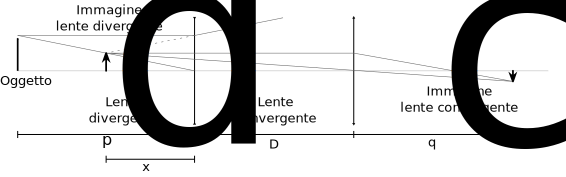
\includegraphics[width=16cm]{drawing2.pdf}
\end{figure}

%questa non è la figura con le freccette in fondo alla pagina? [STESSA FIGURA PRECEDENTE CON AGGIUNTA LA LENTE DIVERGENTE TRA LA SORGENTE E LA LENTE DIVERGENTE]
% PS che diamine state dicendo? lente Div, tra lente Div e sorgente? quante lenti Div abbiamo? LOL

Quindi indicando con:
\begin{itemize}
	\item{$p\ped{d}\,\,$ la distanza tra la sorgente luminosa e il centro della lente divergente;}
	\item{$D\,\,$ la distanza tra le due lenti;}
	\item{$q\ped{c}\,\,$ la distanza tra il centro della lente convergente e l'immagine;}
	\item{$x\,\,$ la distanza incognita tra il centro della lente divergente e l'immagine data da questa;}
\end{itemize}
Il sistema ideato funziona nel seguente modo: la lente divergente produce un'mmagine virtuale tra la sorgente e se stessa. Qusta immagine diventa quindi il nuovo oggetto per la lente convergente che produce un immagine reale sullo schermo. Quindi potendo misurare tutti i parametri sopraelencati ad eccezione di $x$ e $f\ped{d}$ (focale lente divergente) e conoscendo $f\ped{c}$ (focale lente convergente) si può risolvere il seguente sistema

%\begin{equation}
%	\frac{1}{f\ped{d}} \,=\, \frac{1}{p\ped{d}} + \frac{1}{x}
%	\frac{1}{f\ped{c}} \,=\, \frac{1}{(D + x)} + \frac{1}{q\ped{c}}
%\end{equation}
\begin{equation}
 \left\{
  \begin{aligned}
    \frac{1}{f\ped{d}} & \,=\, \frac{1}{p\ped{d}} + \frac{1}{x}\\
    \frac{1}{f\ped{c}} & \,=\, \frac{1}{(D + x)} + \frac{1}{q\ped{c}}
  \end{aligned}
\right.
\end{equation}
%
ottenendo i valori di $x$ e $f\ped{d}$. Inoltre per ottenere un valore più accurato di $f\ped{d}$ abbiamo tenuto ferma la distanza $p\ped{d}$ e abbiamo variato la distanza $D$ e quindi anche $q\ped{c}$, per tre volte. Quindi per ogni tripletta abbiamo sfruttato la relazione (\ref{eq:coniugati}) e abbiamo ottenuto tre valori di $f\ped{d}$. Facendone pertanto la media otterremo un valore più accurato di $f\ped{d}$.
Quindi abbiamo ottenuto che: % <-- questo paragrafo è da rielaborare %

\begin{equation}
	x \,=\, (-12 \pm 2) \,\text{cm} \qquad \text{e} \qquad f\ped{d} \,=\, (-20 \pm 7) \,\text{cm}
\end{equation}

Infine anche per questo sistema di lenti abbiamo calcolato il valore della magnificazione nei due modi possibili, cioè indirettamente con i valori $p\ped{d}$, $x$, $D$ e $q\ped{c}$
\begin{equation}
	m \,=\, m_1 \cdot m_2 \,=\, \frac{p_d}{x} \cdot \frac{q_c}{D+x}
\end{equation} %	|m| \,=\, \frac{x}{p\ped{d}} \,=\,
dove $x$ non è altro che il valore di $q\ped{d}$ e direttamente con i valori di $h$\ped{imm}
\begin{equation}
	m \,=\, \frac{h\ped{imm}}{h}
\end{equation}

\begin{table}[H]
    \centering
    \small
    \begin{tabular}{c c c c c c c c}
        \toprule
        $p_d \; [\si{\centi\metre}]$ & $x \; [\si{\centi\metre}]$ & $D \; [\si{\centi\metre}]$ &
        $q_c \; [\si{\centi\metre}] $ & $f_d \; [\si{\centi\metre}]$ & $h\ped{imm} \; [\si{\centi\metre}]$ & $m$\ped{h} & $m$\ped{pq} \\
        \midrule
		30.50 $\pm$ 0.05 & -12 $\pm$ 2 & 23.10 $\pm$ 0.05 & 76.00 $\pm$ 0.05 & -20 $\pm$ 6 & 0.79 $\pm$ 0.01 & 0.87 $\pm$ 0.01 & 0.9 $\pm$ 0.2 \\
		30.50 $\pm$ 0.05 & -12 $\pm$ 2 & 25.20 $\pm$ 0.05 & 67.10 $\pm$ 0.05 & -20 $\pm$ 7 & 0.64 $\pm$ 0.01 & 0.71 $\pm$ 0.01 & 0.7 $\pm$ 0.2 \\
		30.50 $\pm$ 0.05 & -12 $\pm$ 3 & 27.20 $\pm$ 0.05 & 61.60 $\pm$ 0.05 & -20 $\pm$ 8 & 0.55 $\pm$ 0.01 & 0.61 $\pm$ 0.01 & 0.6 $\pm$ 0.1 \\
        \bottomrule
    \end{tabular}
    \caption{Dati relativi alla lente divergente.}
    \label{tab:div}
\end{table}

%Ovvero conoscendo il valore di $m$ per la lente convergente abbiamo sfruttato la relazione:
%\begin{equation}
%	m \'=\' \frac{h\ped{imm}}{h\ped{ogg}} 
%\end{equation}
%e quindi abbiamo ricavato il valore dell'altezza dell'oggetto per la lente converegente, che però risulta essere nient'altro che l'altezza dell'immagine della lente divergente. Pertanto per ricavare la magnificazione di quest'ultima abbiamo applicato nuovamente la relazione:
%\begin{equation}
%	m \'=\' \frac{h\ped{ogg}}{h} 
%\end{equation}
%e abbiamo ottenuto che $m \'=\' XXX$

\subsection{indice di rifrazione della lente convergente}

Per ricavare il valore dell'indice di rifrazione $n$ della lente convergente non dobbiamo fare altro che sfruttare la seguente relazione:
\begin{equation}
	\text{Legge del costruttore di lenti:} \qquad \frac{1}{f} \,=\, (n-1)\left(\frac{1}{R\ped{1}}-\frac{1}{R\ped{2}}\right)
	\label{eq:costruttore}
\end{equation}
A tal fine abbiamo usato il calibro per misurare i diametro della lente, il suo spessore al centro e quello al bordo. Tutti questi dati sono necessari in quanto nella legge sopracitata sono necessari i valori di $R\ped{1}$ e $R\ped{2}$ che nel nostro caso hanno valore uguale. $R\ped{1}$ e $R\ped{2}$ non sono altro che le distanze tra il centro della lente e la superficie della stessa. Quindi il problema di ricavare $R\ped{1}$ e $R\ped{2}$ si riduce ad un semplice problema di geometria elementare.
Il valore ottenuto di $R$ è: $R \,=\, XXX$.
Quindi per concludere il valore dell'indice di rifrazione ($n$) della lente convergente risulta essere:

\begin{equation}
	n \,=\, XXX
\end{equation}







